%!TEX root = report.tex
\section{Grafisk fremstilling}\label{sec:artwork}
Under vil den grafiske fremstillingen av Garbage Alert bli beskrevet
sammen med valgene som har blitt gjort. Dette vil illustreres med
skjermskudd.

Den grafiske fremstillingen i spillet er ment å være leken og rettet mot
barn i alle aldre, og er sterkt inspirert av den klassiske spillserien
Advance Wars. Videre har det å holde ting oversiktlig og stort nok til å
trykkes på en berøringsskjerm vært noe vi har hatt spesielt i tankene
når grensesnittet har blitt utformet.

\begin{figure} [H]
\centering
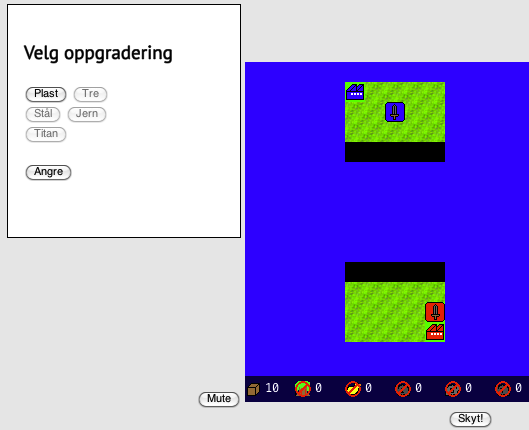
\includegraphics[width=\textwidth]{images/Oppgradering.png}
\caption{Miljøstasjonen kan oppgraderes til å håndtere ulike typer avfallsgjenvinning.}
\label{fig:Oppgradering}
\end{figure}

\begin{figure} [H]
\centering
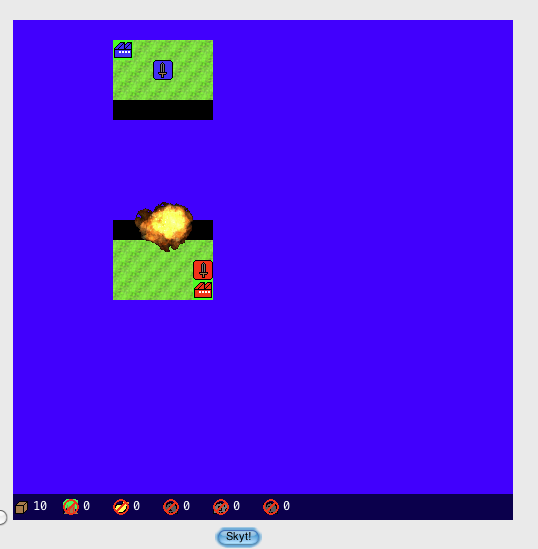
\includegraphics[scale=0.5]{images/Eksplosjon.png}
\caption{Ved et angrep på en annen spiller vil et projektil avfyres og eksplodere på motspillerens eventuelle forsvarsstruktur.}
\label{fig:Eksplosjon}
\end{figure}

\begin{figure} [H]
\centering
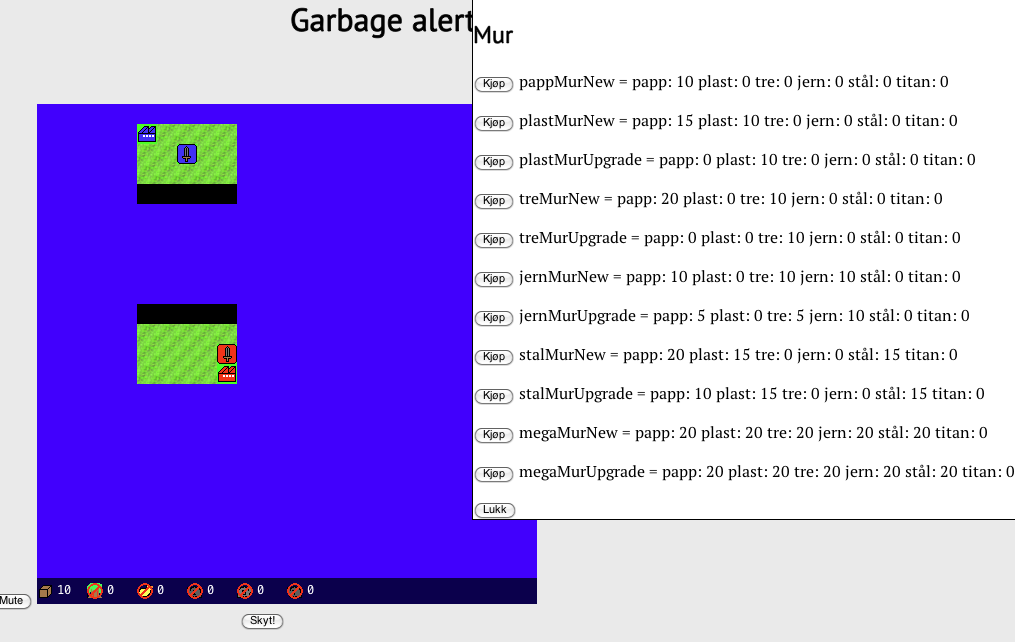
\includegraphics[scale=0.5]{images/OppgradereMur.png}
\caption{Spillerens forsvarsstruktur kan oppgraderes til å håndtere sterkere skyts fra motspilleren, avhengig av tilgjengelige ressurser.}
\label{fig:OppgradereMur}
\end{figure}

\begin{figure} [H]
\centering
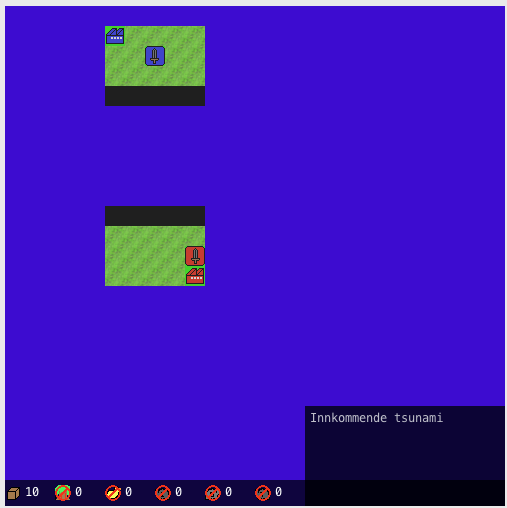
\includegraphics[scale=0.5]{images/Tsunami.png}
\caption{Globale geohasarder kan oppstå som følge av mye global forsøpling, som for eksempel en tsunami.}
\label{fig:Tsunami}
\end{figure}

\begin{figure} [H]
\centering
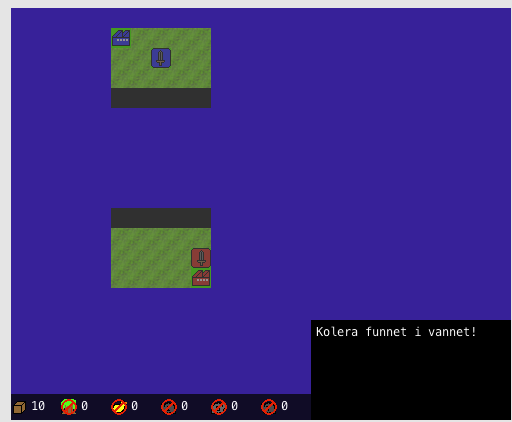
\includegraphics[scale=0.7]{images/Kolera.png}
\caption{Lokale biohasarder kan oppstå som følge av mye lokal forurensning. Her er et sykdomsutbrudd.}
\label{fig:Kolera}
\end{figure}

\begin{figure} [H]
\centering
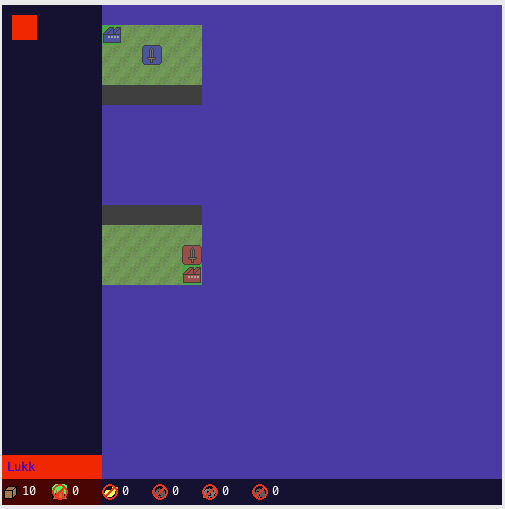
\includegraphics[scale=0.7]{images/OppgradereEnv.png}
\caption{Miljøstasjonens effektivitet kan oppgraderes slik at den gjenvinner mer materialer fra hver avfallsenhet.}
\label{fig:OppgradereEnv}
\end{figure}


Legg merke til at disse skjermskuddene er tatt av en veldig tidlig
prototype som har hatt forkus på å implementere så mye av den tenkte
funksjonaliteten som mulig, heller enn å etablere et konsistent grafisk
uttrykk. Det var ønskelig å benytte så mye som mulig av den kode og
grafikk som ble til i vår tidlige prototype videre i den mer avanserte
prototypen\footnote{Noen vil kanskje si at dette ble gjort i tråd med
landsbyens filosofi om gjenbruk og gjenvinning.}.
